\chapter{Computing Techniques}
The previous chapter demonstrated how the cosmological parameters go into computing the data vectors. But given some data, how does one find the cosmological parameters? From the complexity of the calculations, it's clear that one cannot simply invert the functions to find the associated cosmological parameters. Instead, one would generate a set of cosmological parameters, calculate the data associated with those parameters, then compute the probability of observing the data given the set of parameters. Using this language, it's clear that this computation involves conditional probability densities, so we can use Bayes' theorem to help us determine the parameters.

\section{Markov Chain Monte Carlo}
Markov chains are a step process in which the next step depends solely on the current step~\cite{agrahari_monte_2021}. Formally, a
sequence $X_1,\hdots,X_n$ of random elements is a \textit{Markov Chain} if the conditional distribution  of $X_{n+1}$ depends solely on $X_n$. The set in which $X_i$ take values is called the \textit{state space} of the chain. This is a very abstract definition. However, Markov chains play a regular role in daily life. For example, weather patterns form Markov chains, or the order of words in a sentence. The key here is that, if it rains one day, how likely is it to rain the next day? Or given a word, what is the most probable next word? For a cosmological application, the key is to start with some set of parameters, and slowly move towards the most probable set of parameters.

Bayes' theorem states
\begin{equation}
	P(x|y) = \frac{P(y|x) P(x)}{P(y)}
\end{equation}
Lets set $x=\theta$, the cosmological parameters, and $y=d$, the data vector representing the $3\times 2$ correlation functions, for example. Then
\begin{equation}
	P(\theta|d) = \frac{P(d|\theta) P(\theta)}{P(d)}
\end{equation}
The left-hand side is typically called the \textit{posterior}, while $P(d|\theta)$ is called the likelihood, $P(\theta)$ the prior, and $P(d)$ the evidence. In cosmological notation~\cite{raveri_non-gaussian_2021}, this is usually written
\begin{equation}
	\mathcal{P}(\theta) = \frac{\mathcal{L}(\theta) \Pi(\theta)}{\mathcal{E}}
\end{equation}
The evidence is typically very difficult to compute. One must be able to compute an integral of a complicated function over the entire parameter space (it is possible via techniques such as nested sampling, however these usually take a very long time). Thus, with a given likelihood and prior, it is not feasible to compute the posterior exactly. Markov chain Monte Carlo (MCMC) describes a probabilistic technique that can generate samples from the posterior only using the likelihood and prior and without computing the evidence.
\subsection{The Metropolis-Hastings Algorithm}
The Metropolis-Hastings algorithm~\cite{tobias_metropolis-hastings_nodate,zhao_bayesian_2021,helsby_monte_nodate} is the most common algorithm for doing MCMC. Suppose we want to sample from a distribution $p(x)$. We start with a proposal distribution $g(x_n)$. 
Sample from the proposal distribution to find the next state $x_{n+1}$ with probability $g(x_{n+1}|x_n)$. 
This transition from state $n$ to state $n+1$ must follow the \textit{detailed balance condition}
\begin{equation}
	p(x_n) g(x_{n+1}|x_n) A(x_n \rightarrow x_{n+1}) = p(x_{n+1}) g(x_n|x_{n+1}) A(x_{n+1} \rightarrow x_{n})
\end{equation}
where $A$ is an \textit{acceptance probability}, which I will define more precisely later. 
Using Bayes' Theorem on $p(x)$, the evidence cancels out on each side, 
and thus the detailed balance condition can be simplified to rely solely on the likelihood and prior of $p(x)$, 
which I will denote $\pi$ and $\mathcal{L}$.
\begin{equation}
	\begin{split}
		\pi(x_n)\mathcal{L}(x_n) g(x_{n+1}|x_n) A(x_n &\rightarrow x_{n+1}) = \\
		&\pi(x_{n+1}) \mathcal{L}(x_{n+1}) g(x_{n}|x_{n+1}) A(x_{n+1}\rightarrow x_{n})
	\end{split}
\end{equation}
\begin{equation}
	\Rightarrow \frac{A(x_n \rightarrow x_{n+1})}{A(x_{n+1}\rightarrow x_{n})} = \frac{\pi(x_{n+1}) \mathcal{L}(x_{n+1}) g(x_{n}|x_{n+1})}{\pi(x_n)\mathcal{L}(x_n) g(x_{n+1}|x_n)} \equiv R_{n,n+1}
\end{equation}
This allows us to define the acceptance probability as
\begin{equation}
	A(x_n \rightarrow x_{n+1}) = \min( 1, R_{n,n+1} )\,.
\end{equation}
This probability is used to determine whether the chain moves to $x_{n+1}$ or stays at $x_n$. The chain converges when it reaches a stationary state.

There are a few properties that can be observed for this algorithm:
\begin{itemize}
    \item Having an asymmetrical proposal $g(x)$ can allow for faster convergence of the chain.
    \item The initial sampling may not accurately reflect samples for $p(x)$. 
    This is regarded as the `burn-in' and is generally discarded from the samples.
    \item MCMC sampling loses sampling power for multi-modal distributions. 
\end{itemize}

\section{Tension Metrics}\label{sec:tension_metrics}
Given the 5-dimensional parameter space, there is great difficulty in computing the tension between two measurements. If the data is projected onto one parameter, this can hide the true separation in parameter space (see figure for a Gaussian example). Thus, one needs a method to compute the tension in the full parameter space. In addition, posterior distributions are not generally Gaussian, further increasing the complexity. There are many metrics used to measure tension~\cite{lemos_assessing_2021}, each with different assumptions and consequences.
\subsection{Parameter-based Metrics}
\subsubsection{Metric 1: Parameter Difference}
The main idea of this metric is that if two data sets largely agree, the difference posterior will be centered at 0, so the mass of the posterior above $\mathcal{P}(0)$ will be close to zero. To formalize this notion, start by sampling from the posteriors $\mathcal{P}(\theta_A)$ and $\mathcal{P}(\theta_B)$.
Define $\Delta\theta = \theta_A - \theta_B$. Under this reparameterization, the two posteriors are $\mathcal{P}(\theta_A)$ and $\mathcal{P}(\theta_A-\Delta\theta)$. If the posteriors are independent, one can marginalize over $\theta_A$ to get the parameter difference distribution.
\begin{equation}
    \mathcal{P}(\Delta\theta) = \int \mathcal{P}(\theta_A)\mathcal{P}(\theta_A - \Delta\theta) d\theta_A
\end{equation}
Thus, we can approximate the tension as the volume of the posterior contours with $\mathcal{P}(\Delta\theta)>\mathcal{P}(0)$.
\begin{equation}
    \mathrm{PTE} = \int\limits_{\mathcal{P}(\Delta\theta)>\mathcal{P}(0)}\mathcal{P}(\Delta\theta) d\Delta\theta
\end{equation}
This comes with the benefit of only requiring independent parameter sampling. It makes no assumption of the Gaussianity of the posterior or the likelihood. The difficulty here, however, is actually determining $\mathcal{P}(\theta)$. There are multiple methods used, the most novel of which is discussed later.

\subsubsection{Metric 2: Parameter Difference in Update Form}
As discussed above, we can compute the parameter $Q_{\mathrm{UDM}}$ by
\begin{equation}
    Q_{\mathrm{UDM}} = {(\mu_A - \mu_{A+B})}^T{(C_A-C_{A+B})}^{-1}(\mu_A - \mu_{A+B}) 
\end{equation}
The difference of means is precisely the mean of the parameter difference distribution, and we are using the covariance $C_A+C_{A+B}$.
Thus, it is clear $Q_{\mathrm{UDM}}$ is $\chi^2$ distributed with degrees of freedom given by $\rank(C_A-C_{A+B})$. 
It is clear, however, that this metric relies on the parameter difference to be Gaussian distributed because of its reliance on $Q_{\mathrm{UDM}}$ being $\chi^2$ distributed. Despite this, we proceed anyway. With proper calibration, this metric can be useful even for non-Gaussian posteriors.

\subsubsection{Metric 3: Goodness of Fit Degradation}
For this metric, first find the \textit{maximum a posteriori}, the point $\hat\theta$ that maximizes the posterior. Then compute the likelihood $\mathcal{L}(\hat\theta)$. Lastly, compute the difference in likelihoods between the sum of chain $A$ and $B$ and the joint chain $A+B$
\begin{equation}
	Q_{\mathrm{DMAP}} = 2\mathcal{L}_A(\hat\theta_A) + 2\mathcal{L}_B(\hat\theta_B) - 2\mathcal{L}_{A+B}(\hat\theta_{A+B})
\end{equation}
$Q_{\mathrm{DMAP}}$ is again $\chi^2$-distributed. The interesting part here is how to determine the number of degrees of freedom. The likelihood function, which is on data-space, has degrees of freedom of approximately $1500$ for LSST, but we give it an input of cosmological parameters which belong to a 5 dimensional parameter space. The number of degrees of freedom is related to the number of parameters that are constrained by the likelihood. This can be found by examining the ratio of the variance in the posterior to the variance in the prior; a large ratio of $\mathcal{O}(1)$ means a parameter in not constrained by the likelihood and a ratio $\ll 1$ means a parameter is well constrained by the likelihood. Thus, we define the number of degrees of freedom as
\begin{equation}
	d = N-\mathrm{tr}(C_\Pi^{-1}C_\mathcal{P})
\end{equation}

\subsubsection{Metric 4: Eigentension}
This metric differs from the others by restricting our parameters to ones that are well-measured. We do this as follows:
\begin{enumerate}
	\item Diagonalize the covariance matrix on one of our data sets.
	\item Take the ratio of the variance in the prior to the variance in the posterior and apply an \textit{ad hoc} cut to determine which eigenmodes are well-measured (generally 100 is a good choice).
	\item Project the other data set onto the eigenmodes.
	\item Compute the tension using one of the previous methods.
\end{enumerate}
The idea is that one should not include poorly measured eigenmodes in our tension analysis because the difference is dominated by the prior rather than the likelihood.
\subsection{Evidence-Based Metrics}
\begin{itemize}
	\item Bayesian evidence ratio given by
	\begin{equation}
		R = \frac{\mathcal{E}_{AB}}{\mathcal{E}_A\mathcal{E}_B}
	\end{equation}
	Where $A$ and $B$ are data sets. This method can be written many ways using Bayes' theorem, which will make it apparent that this metric depends heavily on the prior volume.
    \item Bayesian suspiciousness. This metric attempts to remove the dependence on the prior volume by defining the suspiciousness as 
	\begin{equation}
		\log S = \log R - \log I
	\end{equation}
	Of particular interest here is the new value $I$ which is the information ratio, which is defined in terms of the KL divergence.
	\begin{equation}
		\log I = \mathcal{D}_A + \mathcal{D}_B - \mathcal{D}_{AB}
	\end{equation}
	\begin{equation}
		\mathcal{D} = \int \mathcal{P} \log(\frac{\mathcal{P}}{\Pi})
	\end{equation}
\end{itemize}
\subsection{Interpreting the Results}
Given some probability $P$ of a parameter shift, the following formula can give you the number of standard deviations if the probability shift comes from a Gaussian distribution,
\begin{equation}
	n_\sigma = \sqrt{2} \text{Erf}^{-1}(P)\,.
\end{equation}
However we don't have any concrete reason to believe $P$ comes from a Gaussian distribution in general. However, it does come from a Gaussian distribution when the posteriors are Gaussian; thus we can do a test of the metrics by taking two unit Gaussian posteriors and fixing the separation between them. In fact, this example can be computed analytically.
\begin{equation}
    \begin{split}
	\mathcal{P}(\Delta \theta) &= \frac{1}{2\pi} \int\limits_{-\infty}^{\infty} e^{-\theta^2/2} e^{-{(\theta-\Delta\theta)}^2/2}  d\theta \\
				  			   &= \frac{1}{2\pi} \cdot \sqrt{\pi} e^{-{(\Delta\theta)}^2/4}\\
				   			   &= \frac{1}{\sqrt{4\pi}}e^{-{(\Delta\theta)}^2/4}\\
    \end{split}
\end{equation}
The parameter difference posterior is a Gaussian with standard deviation $\sqrt{2}$. The separation is fixed by $a$, hence the shift is $\mathcal{P}(a)$. Hence, the shift probability is
\begin{equation}
	\Delta = \int\limits_{-a}^{a} e^{-{(\Delta\theta)}^2/4} d\Delta\theta\,.
\end{equation}
We can compare the analytic result to the computational result for each of the metrics to see which ones are most accurate. In practice, this integral is computed with Monte-Carlo integration, where the error is evaluated using the Clopper-Pearson interval on the binomial distribution.
\subsection{DES versus Planck Results}
A subset of these exercises have been performed previously by the Dark Energy Survey (DES) against the Planck results. In~\cite{lemos_assessing_2021}, Lemos et al. generates an a-priori tension on the cosmological parameters by shifting the DES fiducial cosmology along $\sigma_8$ and $\Omega_m$. They approximate the a-priori tension using the Gaussian approximation,
\begin{equation}\label{eq:a-priori}
	\chi^2 = \delta\theta (C_\mathrm{DES}+C_\mathrm{Planck})\delta\theta
\end{equation}
where $\delta\theta$ is $(\sigma_8,\Omega_m)$ and $C$ the covariance of DES and Planck, respectively.

They then compute the tension metrics and compare to the a-priori Gaussian tension. The main result demonstrates what the resulting tension is from a fixed shift along a single parameter. Their result is presented in this thesis in figure~\ref{fig:planck_des_tension}. An additional note is that Gaussian tension tends to underestimate the tension presented in other metrics, highlighting the importance of capturing non-Gaussianities.
\begin{figure}[tb]
	\centering
	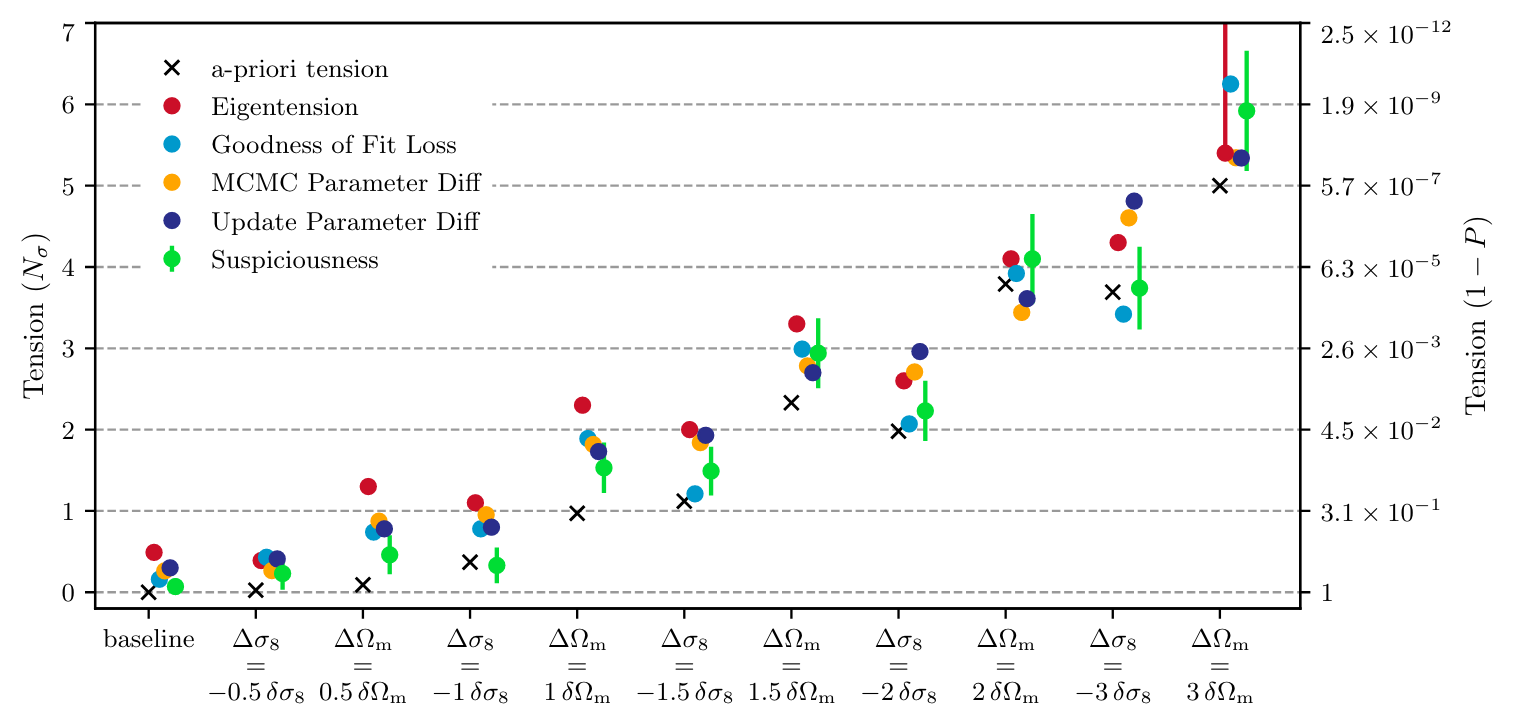
\includegraphics[width=0.9\textwidth]{plots/planck_des_result.png}
	\caption{Result of tension metrics between Planck and DES (figure 6 in~\cite{lemos_assessing_2021}). A-priori tension is the Gaussian approximation described in equation~\ref{eq:a-priori}.}
	\label{fig:planck_des_tension}
\end{figure}
\section{Normalizing Flows}
The method of normalizing flows (MAF) implemented here uses Masked Autoencoders for Density Estimation (MADE) to construct the flow~\cite{germain_made_2015,papamakarios_masked_2018,raveri_non-gaussian_2021}. 
Suppose we have an input to the flow $x_i$. 
The output of the map is $y_i= \mu(x_{1:i-1})+\sigma(x_{1:i-1})x_i$. 
The $\mu$ and $\sigma$ are found using neural networks which receive masked inputs $x_{1:i-1}=(x_1,\ldots,x_{i-1},0,\ldots,0)$. 
Since the input depends solely on the first $i-1$ inputs, the normalizing flow is \textit{autoregressive} and the Jacobian is triangular.

The implementation in \textsc{TensorFlow} uses \textit{bijectors}, a local diffeomorphism between a manifold $M$ and a target manifold $N$ (which are our parameter spaces), i.e., $\phi:M\rightarrow N$ such that $\phi$ is differentiable and injective. 
In \textsc{TensorFlow}, bijectors have three operations, forward, inverse, and log\_det\_jacobian, which are precisely the three we want. 
By constructing a bijector for each masked input, the full normalizing map can be constructed.

An intuitive way to think of normalizing flow is as a reparameterization. Consider our posterior as a manifold $X$. The manifold is constructed via the parameterization with charts $\phi_i:X\rightarrow U_i \subset \mathbb{R}^n$ for $i$ in indexing set $I$. 
The charts determine the atlas $A = \bigsqcup\limits_{i\in I} (U_i,\phi_i)$. 
The goal is to determine a new parameterization for $X$ given by the charts $\psi_j:X\rightarrow V_j \subset \mathbb{R}^n$ in which samples in $X$ are Gaussian distributed. 
Let $Y \subset X$ be given by $Y = \phi_i^{-1}(U_i) \cap psi_j^{-1}(V_j)$. 
Then the transition function is given by $\tau:\phi_i(Y)\rightarrow\psi_j(Y)$. 
To ensure our parameterizations are diffeomorphic, $\tau$ is required to be differentiable and its inverse differentiable 
(in fact, we are working with smooth reparameterizations so the transition function and its inverse should be smooth).

The next question one may have is, `what do flows have to do with this?' Above, the concept of normalizing flows is described as a reparameterization, but there is another good description involving flows. Again, let $X$ be our parameter space, the graph $(\theta,\mathcal{P}(\theta))$, and $TX$ the tangent bundle of $X$. Each MAF can be though of as a finite sequence of vector fields $v_i:X \rightarrow TX$. Each point is moved along its integral curve determined by each $v_i$. What is great about this definition is that it immediately implies an MAF is a diffeomorphism. 
\begin{prop}
Suppose $v:X \rightarrow TX$ is a vector field on $X$ and $x \in X$. Then for any $\epsilon>0$ there exists a unique function $f:B[-\epsilon,\epsilon]\rightarrow X$ such that $f$ is an integral curve of with infinitesimal generator $v$ and with $f(0) = x$.  
\end{prop}
\begin{proof}
Given a vector $v_x:U\rightarrow T_x X$ with $x\in U$, for it to be in the tangent space $T_pX$ it must have a curve with $f(0)=x$ and $f'(0)=v_x$. This follows from the definition of $T_xX$.

Suppose there are two such curves, $\alpha$ and $\beta$ both mapping from $I=(-\epsilon,\epsilon)$ to $X$ and with $\alpha(0) = x = \beta(0)$ and both with $\alpha'(0) = v_x = \beta'(0)$. Then they both solve the system of autonomous ODEs for $i=1,\dots,n$
\begin{equation}
\begin{split}
	\dot{\gamma}^i(t) &= v^i(\gamma(t)) \\
	\gamma^i(0) &= c^i
\end{split}
\end{equation}
This can be solved by $\gamma^i(t) = \int\limits_{U\subset X}v^i(\gamma(t))\text{vol.}$. Since $v$ is a tangent vector field, there exists a curve $\phi$ with $\phi' = v$, so the solution is $\gamma^i(t) = \phi^i(t)+C^i$. The integration constants are fixed by the initial condition $C^i=-c^i$, hence any two functions satisfying this system of ODE's, including $\alpha$ and $\beta$, are equivalent for all $t\in I$.
\end{proof}
Autoregressive models have several pitfalls that we would like to avoid in this project. Namely, autoregressive models are sensitive to the order of the input, however our result does not have any dependence. 
\begin{figure}[ht]
	\centering
	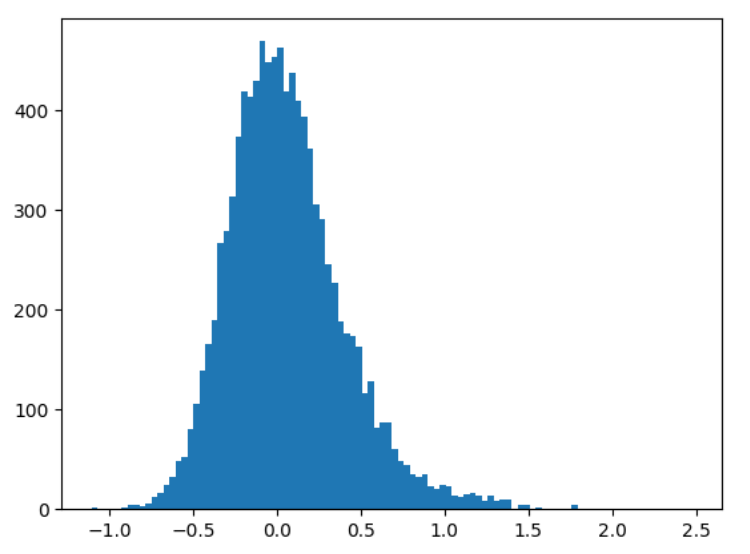
\includegraphics[width=0.9\textwidth]{plots/t=1.png}
	\caption{An example non-Gaussian distribution (non-zero skewness).}
	\label{fig:non-gauss}
\end{figure}
\begin{figure}[ht]
	\centering
	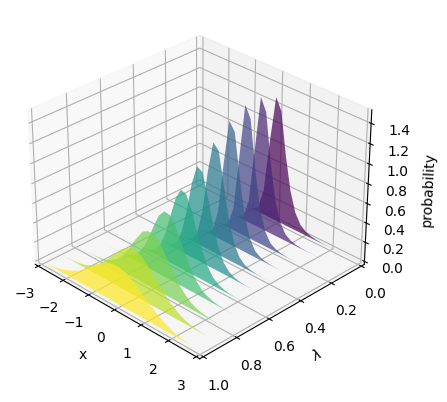
\includegraphics[width=0.9\textwidth]{plots/3d_flow.png}
	\caption{An example of normalizing flow as the transformation is `turned on', represented by the parameter $\lambda$. The non-Gaussian distribution at $\lambda=0$ is transformed into the Gaussian distribution at $\lambda=1$.}
	\label{fig:NF}
\end{figure}